\chapter{Results}

\section{Envelope Variants}

\begin{figure}[H]
\centering
	\begin{subfigure}[b]{0.45\textwidth}
		\centering
		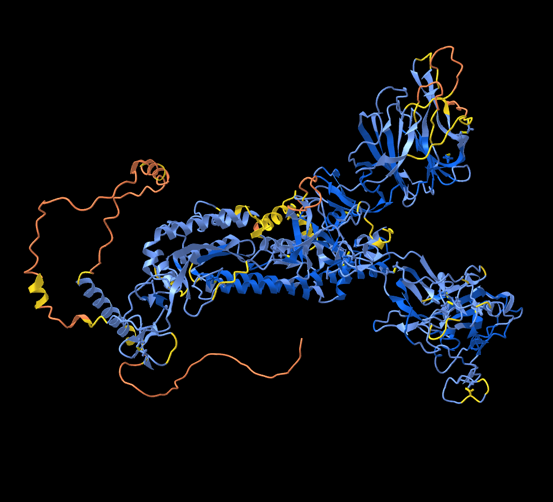
\includegraphics[width=\textwidth]{figures/gu280_ref.png}
		\caption{Left part of a figure partitioned into subfigures.}
		\label{plddtCon2a}
	\end{subfigure}
	\hfill
	\begin{subfigure}[b]{0.49\textwidth}
		\centering
		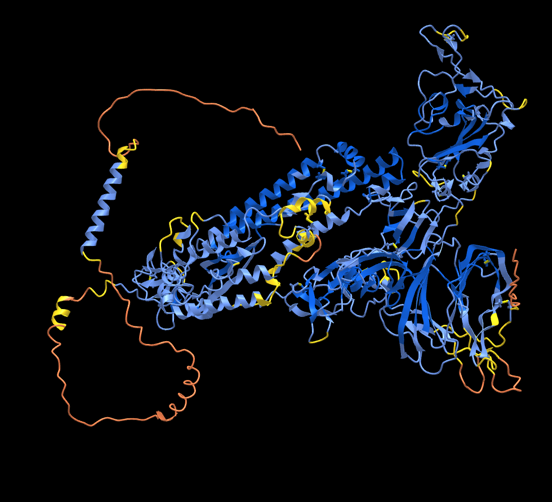
\includegraphics[width=\textwidth]{figures/gu280_var3.png}
		\caption{Right part of a figure partitioned into subfigures.}
		\label{plddtCon2b}
	\end{subfigure}
	\caption{An example of a subdivided figure.}
	\label{subfigure_this}
\end{figure}

As we have labeled the above figure containing subfigures, we can reference it using \ref{subfigure_this}.

\begin{figure}[H]
	\centering
	\fbox{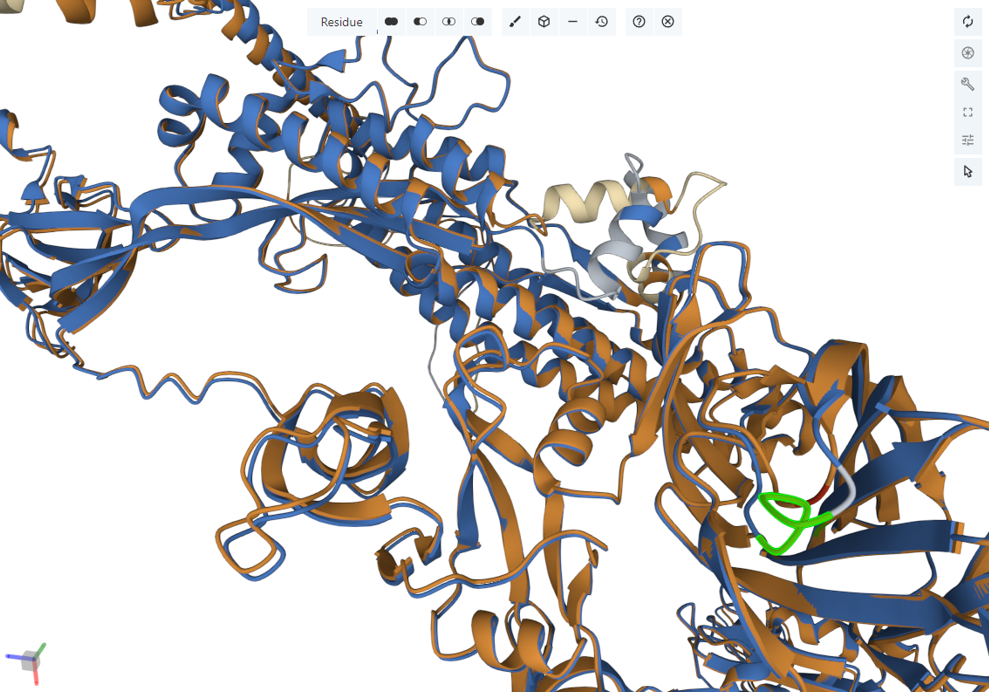
\includegraphics[width=0.9\textwidth]{figures/gu280_var3_comp_close.png}}
	\caption{An example of an unsubdivided figure.}
	\label{figured_out}
\end{figure}

Similarly, we can reference the unsubdivided figure using \ref{figured_out}.

\section{Code Example}

The results of the study include the generated data, outcomes of statistical tests, and visual evaluations such as plant leaf imagery. This section focuses on presenting these results objectively without interpretation. Incremental values can be depicted using tables and figures where necessary.

Below is an example of how to insert an algorithm in LaTeX:

\begin{algorithm}[H]

\KwData{
\begin{itemize}
    \item $g$: The GO term to compute the mutation probability lookup table for.
    \item $\mathcal{H}$: The \emph{ordered} set of homologous protein pairs $p_i$, where\\
    \hspace{1cm} at least one member has annotation $g$,\\
    \hspace{1cm} with $\mathcal{G}_x$ as the set of GO term annotations of protein $x$: \\
    \hspace{1cm} $p_i = \{ \, p_i^1, p_i^2 ~ | ~ \exists ~ k \in \{1,2\} : g \in \mathcal{G}_{p_i^k} \, \}$, and\\
    \hspace{1cm} each pair $p_i$ has a sequence distance $d_i$ such that: $d_{i-1} \leq d_i$.
\end{itemize}
}
\KwResult{
\begin{itemize}
    \item $M$: Ordered set of mutation probabilities $P( \, g^{mut} \,|\, d_k \,)$, with\\
    \hspace{1cm} $m_{k-1} \leq m_k$ for $d_{k-1} \leq d_k$.
\end{itemize}
}

\BlankLine
\textbf{Initialize:}\\
$n_{not\_sharing} \leftarrow 0$\\
$n_{all} \leftarrow 0$\\
$m_{candidate} \leftarrow 0$\\
$m_{current} \leftarrow 0$\\
\BlankLine

\ForEach{$p_i \in \mathcal{H}$, $1 \leq i \leq |\mathcal{H}|$}{
    Increment $n_{all}$ by 1.\\
    \If{$\exists ~ k \in \{1,2\} : g \notin \mathcal{G}_{p_i^k}$}{
        Increment $n_{not\_sharing}$ by 1.\\
    }
    $m_{candidate} \leftarrow \frac{n_{not\_sharing}}{n_{all}}$\\
    \If{$m_{candidate} > m_{current}$}{
        $m_{current} \leftarrow m_{candidate}$\\
        Append $m_{current}$ to $M$.\\
    }
}
\caption{Mutation Probability Lookup Algorithm}
\label{alg:mutation_lookup}
\end{algorithm}


\section{Example of using a reference to another section}

This is a reference example. To reference the code example above, simply use \\
\verb|\ref{alg:mutation_lookup}| \ref{alg:mutation_lookup}.

Find more information about the materials in section \ref{Topics_of_Material} \\
(\verb|\ref{Topics_of_Material}|) on page \pageref{Topics_of_Material}
(\verb|\pageref{Topics_of_Material}|).
